%%
\bigheading{Critical Projects}
\authors{Gyula Horváth}{Gyula Horváth}{Gyula Horváth}

Consider the graph model of the problem: a directed graph $G=(V,E)$ where $V$ is the set of the subprojects, $V=\{1, \ldots ,N \} $ and the edges of G are pairs $(u,v)$ if $u$ precedes $v$.
G is obviously acyclic graph. Consider the layer decomposition of the node set V. \\
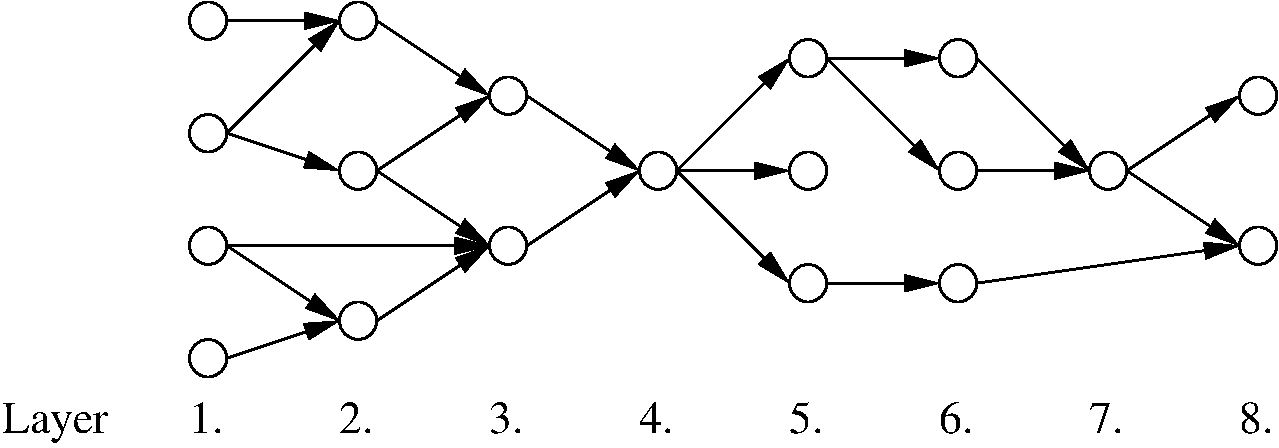
\includegraphics[height=4cm]{img/abra21.pdf}

The first layer contains all nodes of indegree 0. Delete all nodes of the first layer, then all nodes of  0 indegree in this graph are the members of the second layer, and so on.
Denote the layer number of node $p$ by $L(p)$. Therefore the following holds.
\begin{eqnarray}
L(p) = \left\{
\begin{array}{lll}
 1 & \textrm{ if } indegree(p)=0\\
 \max \{ L(q): q \rightarrow p \in E\} +1 & \textrm { if } indegree(p)>0
\end{array}\right.
\end{eqnarray}
We define the function $F$ as follows.
\begin{eqnarray}
F(p) = \left\{
\begin{array}{lll}
 \infty & \textrm{ if } outdegree(p)=0\\
 \min \{ L(q): p \rightarrow q \in E\} & \textrm { otherwise }
\end{array}\right.
\end{eqnarray}
Define the function $Ln(x)$ as the number of nodes in the layer $x$.
\[ Ln(x)= \vert \{p: L(p)=x \} \vert\]
\subsection*{Statement}
A node $p$ is critical if and only if the following two conditions hold.

\[ Ln(L(p))=1 \]
\[ (\forall q)(L(q)<L(p) \Rightarrow F(q) \leq L(p)) \]

\noindent Assume that the conditions hold for a node $p$. We will show that for all node $q$ if $L(p)<L(q)$ then there is path from $p$ to $q$ and if $L(q)<L(p)$ then  there is path from $q$ to $p$. \\
From the first condition and the definition of the function $L()$ it follows that for all nodes $q$ with $L(p)<L(q)$ there is path from $p$ to $q$: $p \rightsquigarrow q$. \\
Let $L(q)<L(p)$. We prove by induction on $L(q)$ that there is path from $q$ to $p$. If $L(p)=L(q)+1$ then by the definition of $L$ and the second condition it follows that there is an edge from $q$ to $p$. Assume that $L(q)=k$ and for all nodes $s$ such that $k<L(s) \leq L(p)$ there is a path from $s$ to $p$. It follows from the second condition that there is a node $s$ such that  $L(s) \leq L(p)$ and there is an edge from $q$ to $s$. Therefore there is path $q \rightarrow s \rightsquigarrow p$.\\

Conversely, assume that $p$ is critical. This implies that $p$ must be the only node in its layer, that is the first condition holds. Assume that $L(q)<L(p)$ and $F(q) > L(p)$. This is a contradiction, because there is a path $q \rightsquigarrow p$.\\

Therefore if we compute the function $L$ and $F$ we can determine all critical nodes.\\
In order for checking the second condition, we compute a topological order $T=p-1,\ldots, p_n$ with the following property that for all nodes $p$ and $q$ if $L(p)<L(q)$ it follows that $p$ precedes $q$ in the topological order. This can be done in $\Theta(n+m)$ time when $n$ id the number of nodes and $m$ is the number of edges of the graph.\\
\emph{\textbf{Running time of the algorithm}}: $O(n+m)$

